\documentclass{article}
\usepackage{amsmath,amssymb}
\usepackage{fullpage}
\usepackage{mathrsfs}
\usepackage{setspace}
\usepackage{graphicx}
\usepackage{listings}
\usepackage{multirow}
\renewcommand{\baselinestretch}{1}
\pagestyle{empty}
\usepackage{color}
\definecolor{dkgreen}{rgb}{0,0.6,0}
\definecolor{gray}{rgb}{0.5,0.5,0.5}
\definecolor{mauve}{rgb}{0.58,0,0.82}

\lstset{frame=tb,
	language=Matlab,
	aboveskip=3mm,
	belowskip=3mm,
	showstringspaces=false,
	columns=flexible,
	basicstyle={\small\ttfamily},
	numbers=none,
	numberstyle=\tiny\color{gray},
	keywordstyle=\color{blue},
	commentstyle=\color{dkgreen},
	stringstyle=\color{mauve},
	breaklines=true,
	breakatwhitespace=true,
	tabsize=4
}
\begin{document}
\noindent{\bf Homework 5}

\noindent{\bf Jingmin Sun}

\noindent{\bf 661849071}


\begin{enumerate}
\item
\begin{enumerate}

\item
\begin{enumerate}
\item
For direct method, we can get the formula of \[P_3(x) = a_0+a_1x+a_2x^2+a_3x^3\]
Since $P_3(x_j) = y_j$, for $j = 1,2,3,4$, \begin{align*}
A\begin{bmatrix}
a_0\\a_1\\a_2\\a_3
\end{bmatrix} &=\begin{bmatrix}
6\\4\\3\\-6
\end{bmatrix}\\
\mbox{where }\; A &=\begin{bmatrix}
1&x_1&x_1^2&x_1^3\\
1&x_2&x_2^2&x_2^3\\
1&x_3&x_3^2&x_3^3\\
1&x_4&x_4^2&x_4^3\\
\end{bmatrix}\\
&=\begin{bmatrix}
1&-1&1&-1\\
1&1&1&1\\
1&2&4&8\\
1&3&9&27
\end{bmatrix}\\
\therefore \begin{bmatrix}
1&-1&1&-1\\
1&1&1&1\\
1&2&4&8\\
1&3&9&27
\end{bmatrix}\begin{bmatrix}
a_0\\a_1\\a_2\\a_3
\end{bmatrix} &=\begin{bmatrix}6\\4\\3\\-6
\end{bmatrix}\\
\end{align*}
And by Matlab we can get:
\lstinputlisting[language=Matlab,caption={Result}]{11.txt}
so \[a_0 = 3, a_1 = 0, a_2 =2, a_3 =-1\] which means $P_3(x) = 3+2x^2-x^3$
\item
For Lagrange Approach, we have the formula of \[P_3(x) = \sum_{j=1}^4 y_j l^{(j)}(x)\] So, our goal is to find $l^{(j)}(x)$, since \begin{align*}
l^{(1)}(x) &=\dfrac{{(x-x_2)(x-x_3)(x-x_4)}}{(x_1-x_2)(x_1-x_3)(x_1-x_4)}\\
&=\dfrac{{(x-1)(x-2)(x-3)}}{(-2)(-3)(-4)}\\
&=-\dfrac{(x-1)(x-2)(x-3)}{24}\\
l^{(2)}(x) &=\dfrac{{(x-x_1)(x-x_3)(x-x_4)}}{(x_2-x_1)(x_2-x_3)(x_2-x_4)}\\
&=\dfrac{{(x+1)(x-2)(x-3)}}{(2)(-1)(-2)}\\
&=\dfrac{(x+1)(x-2)(x-3)}{4}\\
l^{(3)}(x) &=\dfrac{{(x-x_1)(x-x_2)(x-x_4)}}{(x_3-x_1)(x_3-x_2)(x_3-x_4)}\\
&=\dfrac{{(x+1)(x-1)(x-3)}}{(3)(1)(-1)}\\
&=-\dfrac{(x+1)(x-1)(x-3)}{3}\\
l^{(4)}(x) &=\dfrac{{(x-x_1)(x-x_2)(x-x_3)}}{(x_4-x_1)(x_4-x_2)(x_4-x_3)}\\
&=\dfrac{(x+1)(x-1)(x-2)}{(4)(2)(1)}\\
&=\dfrac{(x+1)(x-1)(x-2)}{8}\\
\end{align*}
Thus,\begin{small}
\begin{align*}
P_3(x)& = -6\dfrac{(x-1)(x-2)(x-3)}{24}+4\dfrac{(x+1)(x-2)(x-3)}{4}-3\dfrac{(x+1)(x-1)(x-3)}{3}-6\dfrac{(x+1)(x-1)(x-2)}{8}\\
& = -\dfrac{(x-1)(x-2)(x-3)}{4}+(x+1)(x-2)(x-3)-(x+1)(x-1)(x-3)-\dfrac{3(x+1)(x-1)(x-2)}{4}
\end{align*}
\end{small} 
\item
For Newton Divided difference, we can get the form of \[P_3(x) = \boxed{ }+\boxed{ }\;(x-x_1)+\boxed{ }\;(x - x_1)(x-x_2) +\boxed{ }\; (x-x_1)(x-x_2)(x-x_3) \] And for the coefficient, we can make a table for it:

\begin{small}
\begin{tabular}{|c|c|c|c|c|}
\hline
$x_1=-1$&$g[x_1] = y_1 =6$&&&\\
\hline
$x_2=1$&$g[x_2] = y_2 =4$&$g[x_1,x_2] = \dfrac{4-6}{1-(-1)} = -1$&&\\
\hline
$x_3=2$&$g[x_3] = y_3 =3$&$g[x_2,x_3] = \dfrac{3-4}{2-1} = -1$&$g[x_1,x_2,x_3] =\dfrac{-1-(-1)}{2-(-1)} =0$&\\
\hline
\multirow{2}*{$x_4=3$}&\multirow{2}*{$g[x_4] = y_4 =-6$}&\multirow{2}*{$g[x_2,x_3] = \dfrac{-6-3}{3-2} = -9$}&\multirow{2}*{$g[x_2,x_3,x_4] =\dfrac{-9-(-1)}{3-1} =-4$}&$g[x_1,x_2,x_3,x_4] $ \\~&~&~&~&$= \dfrac{-4-0}{3-(-1)} = -1$\\
\hline
\end{tabular}
\end{small}

Thus,\begin{align*}
P_3(x) &= 6-(x-x_1)- (x-x_1)(x-x_2)(x-x_3) \\
&= 6-(x+1)- (x+1)(x-1)(x-2) 
\end{align*}
\end{enumerate}
\item
\begin{align*}
g(x)&=\begin{cases}g_1(x)&x\in[-1,1]\\g_2(x)&x\in(1,2]\\g_3(x)&x\in(2,3]\\\end{cases}\\
&=\begin{cases}a_1x+b_1&x\in[-1,1]\\a_2x+b_2&x\in(1,2]\\a_3x+b_3&x\in(2,3]\\\end{cases}\\
\therefore a_1\cdot (-1)+b_1 &=6\\
a_1\cdot 1+b_1 &=4\\
a_2\cdot 1+b_2 &=4\\
a_2\cdot 2+b_2 &=3\\
a_3\cdot 2+b_3 &=3\\
a_3\cdot 3+b_3 &=-6\\
\therefore a_1=-1,b_1 =5,a_2=-1,&b_2=5,a_3=-9,b_3=21\\
g(x)&=\begin{cases}-x+5&x\in[-1,1]\\-x+5&x\in(1,2]\\-9x+21&x\in(2,3]\\\end{cases}\\
&=\begin{cases}-x+5&x\in[-1,2]\\-9x+21&x\in(2,3]\\\end{cases}\\
\end{align*}
\item
We can use direct method here, such that 
\[P_6(x) = a_0+a_1x+a_2x^2+a_3x^3+a_4x^4+a_5x^5+a_6x^6\]
Since $P_6(x_j) = y_j$, for $j = 1,2,3,4$, \begin{align*}
A\begin{bmatrix}
a_0\\a_1\\a_2\\a_3\\a_4\\a_5\\a_6
\end{bmatrix} &=\begin{bmatrix}
6\\4\\3\\-6
\end{bmatrix}\\
\mbox{where }\; A &=\begin{bmatrix}
1&x_1&x_1^2&x_1^3&x_1^4&x_1^5&x_1^6\\
1&x_2&x_2^2&x_2^3&x_2^4&x_2^5&x_2^6\\
1&x_3&x_3^2&x_3^3&x_3^4&x_3^5&x_3^6\\
1&x_4&x_4^2&x_4^3&x_4^4&x_4^5&x_4^6\\
\end{bmatrix}\\
&=\begin{bmatrix}
1&-1&1&-1&1&-1&1\\
1&1&1&1&1&1&1\\
1&2&4&8&16&32&64\\
1&3&9&27&81&243&729
\end{bmatrix}\\
\therefore \begin{bmatrix}
1&-1&1&-1&1&-1&1\\
1&1&1&1&1&1&1\\
1&2&4&8&16&32&64\\
1&3&9&27&81&243&729
\end{bmatrix}\begin{bmatrix}
a_0\\a_1\\a_2\\a_3\\a_4\\a_5\\a_6
\end{bmatrix} &=\begin{bmatrix}6\\4\\3\\-6
\end{bmatrix}\\
\end{align*}
To solve the linear system, we can put it into an augmented matrix and reduced it to the "diagonal " form:
And by Matlab we can get:
\lstinputlisting[language=Matlab,caption={Result}]{12.txt}
And we can get for all $\begin{bmatrix}
a_0\\a_1\\a_2\\a_3\\a_4\\a_5\\a_6
\end{bmatrix}\in \mathbb{R}^6$, such that \begin{align*}
a_0+6a_4+30a_5+120a_6&=3\\
a_1-5a_4-19a_5-70a_6&=0\\
a_2-5a_4-30a_5-119a_6&=2\\
a_3+5a_4+20a_5+70a_6&=-1\\
\end{align*}
will be a interpolate of $f(x)$ of degree 6, since $a_6\neq 0$ and one example can be find by setting $a_6=a_5=a_4 =1$, and we can get by matlab that:
\lstinputlisting[language=Matlab,caption={Result}]{13.txt}
Thus $a_0 = -153, a_1 = 94, a_2 = 156, a_3 = -96$, and this example can be written as \[P_6(x) = -153+94x+156x^2-96x^3+x^4+x^5+x^6\]
\end{enumerate}
\item
\begin{enumerate}
\item
Since \begin{align*}
g_1''(x_2) &=g_2''(x_2)\\
3x_2&=2c+6d(x_2-2)\\
3\times 2 &= 2c+0\\
c&=3
\end{align*}
\item
Since spline is natural, so that \begin{align*}
g_2''(x_3)&=0\\
2c+6d(x_3-2)&=0\\
6&=-6d(1)\\
d&=-1
\end{align*}
\end{enumerate}
\item
\begin{enumerate}
\item
Since we have need the degree 2 interpolating polynomial $p(x)$, we can use Lagrange approach with \[p(x) = \sum_{j=1}^3 y_j l^{(j)}(x)\] where \begin{align*}
l^{(1)}(x) &= \dfrac{(x-x_2)(x-x_3)}{(x_1-x_2)(x_1-x_3)}\\
&=\dfrac{(x-2)(x-4)}{(1-2)(1-4)}\\
&=\dfrac{(x-2)(x-4)}{3}\\
l^{(2)}(x) &= \dfrac{(x-x_1)(x-x_3)}{(x_2-x_1)(x_2-x_3)}\\
&=\dfrac{(x-1)(x-4)}{(2-1)(2-4)}\\
&=-\dfrac{(x-1)(x-4)}{2}\\
l^{(3)}(x) &= \dfrac{(x-x_1)(x-x_2)}{(x_3-x_1)(x_3-x_2)}\\
&=\dfrac{(x-1)(x-2)}{(4-1)(4-2)}\\
&=\dfrac{(x-1)(x-2)}{6}\\
\therefore p(x)&=-\dfrac{\ln(2)(x-1)(x-4)}{2}+\dfrac{\ln(4)(x-1)(x-2)}{6}\\
\end{align*}
\item
\begin{align*}
|f(x)-p(x)|&=\left|\dfrac{(x-x_1)(x-x_2)(x-x_3)}{3!}f'''(c)\right|&\mbox{ for } c \in [\min(x,x_1,x_2,x_3), \max(x,x_1,x_2,x_3)]\\
&= \left|2\dfrac{(x-1)(x-2)(x-4)}{6c^3}\right|&\mbox{ for } c \in [\min(x,x_1,x_2,x_3), \max(x,x_1,x_2,x_3)]\\
&= \left|\dfrac{(x-1)(x-2)(x-4)}{3c^2}\right|&\mbox{ for } c \in [\min(x,x_1,x_2,x_3), \max(x,x_1,x_2,x_3)]\\
|f(3)-p(3)|&= \left|\dfrac{(3-1)(3-2)(3-4)}{3c^2}\right|&\mbox{ for } c \in [1, 4]\\
&= \left|\dfrac{-2}{3c^2}\right|&\mbox{ for } c \in [1, 4]\\
&= \left|\dfrac{2}{3c^2}\right|&\mbox{ for } c \in [1, 4]\\
&\leq \dfrac{2}{3}
\end{align*}
\item
\begin{align*}
|f(3)-p(3)|&=\left|\ln(3)-\left(-\ln(2)\cdot\dfrac{(3-1)(3-4)}{2}+\ln(4)\cdot\dfrac{(3-1)(3-2)}{6}\right)\right|\\
&=\left|\ln(3)-\left(-\ln(2)\cdot\dfrac{-2}{2}+\ln(4)\cdot \dfrac{2}{6}\right)\right|\\
&=\left|\ln(3)-\left(\ln(2)+\dfrac{\ln(4)}{3}\right)\right|\\
&= \left|\dfrac{\ln(\frac{27}{32})}{3}\right|\\
&\approx 0.056633
\end{align*}
\end{enumerate}
\item
\begin{enumerate}
\item
Here, we can define $z_j$ as $(x-x_j)$ 
\begin{align*}
p(x)&=a_1+\sum_{j=2}^n a_j(x-x_1)(x-x_2)\cdots(x-x_{j-1})\\
&=a_1+\sum_{j=2}^n a_j\Pi_{i=1}^{i-1}z_i\\
&=a_1+z_1a_2+z_1z_2a_3+\cdots+z_1z_2\cdots z_{n-1}a_n\\
&=a_1+z_1(a_2+ z_2(a_3+ z_3(\cdots a_{n-1}+z_{n-1}(a_n))))\\
&=a_1+(x-x_1)(a_2+ (x-x_2)(a_3+ (x-x_3)(\cdots a_{n-1}+(x-x_{n-1})(a_n))))
\end{align*}
\item
The function to calculate the coefficient of Newton Divided Difference Method: 
 
 \lstinputlisting[language=Matlab, numbers=left, stepnumber=1, firstline=1,caption={myPolyCoef.m function},frame=single]{myPolyCoef.m}
 
 \item
 The function to evaluate the interpolation at point $x$:
 
 \lstinputlisting[language=Matlab, numbers=left, stepnumber=1, firstline=1,caption={myPolyEval.m function},frame=single]{myPolyEval.m}
 \item
 Firstly, the most important property is that $f(x) = p(x) = y$ at the points $\{x_j,y_j\}_{j=1}^n$, so we can choose write a test code for that 
  \lstinputlisting[language=Matlab, numbers=left, stepnumber=1, firstline=1,caption={test\_original.m function},frame=single]{test_original.m}
  and we can check the output:
  \lstinputlisting[language=Matlab,caption={Output}]{original.txt}
  And we can observe that the error is approximately zero, and the error might be caused by the rounding process of computer, so we can conclude that our implementation may be correct.
  
  Besides that, since we know that $n+1$ points can exactly interpolate polynomial of degree n, so I randomly choose coefficients $a_0, a_1 \cdots a_n$ to make a random polynomial $a_0+a_1x+a_2x^2+\cdots a_nx^n$, and use Horner's nested method to  calculate the $y$ for randomly choosen $n+1$ $x$s. And I then randomly choose three points $z_1,z_2,z_3$, and calculate the error between $f(z_i)$ and $p(z_i)$, which interpolated by ${x_j,y_j}$ 
    \lstinputlisting[language=Matlab, numbers=left, stepnumber=1, firstline=1,caption={test\_z.m function},frame=single]{test_z.m}
  and we can check the output:
  \lstinputlisting[language=Matlab,caption={Output}]{polynomial.txt}
  And we can observe that the error is near machine epsilon as well, so we can conclude that our implementation is approximately correct.
  
  Finally, we can check the upper bound for the interpolation  error, with the $\sin$ function, since $\dfrac{d\sin(x)}{dx}\leq 1$ \begin{align*}
  \therefore |f(x) - P_n(x)| &= \left|\dfrac{(x-x_1)(x-x_2)\cdots(x-x_{n+1}))}{(n+1)!}f^{(n+1)}(c)\right|\\
  &\leq  \left|\dfrac{(x-x_1)(x-x_2)\cdots(x-x_{n+1}))}{(n+1)!}\right|\\
  \end{align*}
  \lstinputlisting[language=Matlab, numbers=left, stepnumber=1, firstline=1,caption={test\_sin.m function},frame=single]{test_sin.m}
  And the output follows,
    \lstinputlisting[language=Matlab,caption={Output}]{sin.txt}
    We can see that all the error are bounded by the upperbound, so that the algorithm is correct.
    \item
  I implement the following form to interpolating $f(x) = \dfrac{1}{1+4x^2}$ with uniformly distributed $x \in [-2,2]$:
   \lstinputlisting[language=Matlab, numbers=left, stepnumber=1, firstline=1,caption={uniform.m function},frame=single]{uniform.m}
   And we can get the output
     \lstinputlisting[language=Matlab,caption={Output}]{uniform.txt}
     And from the figure below, $n=6$ on the left, and $n = 13$ on the right, we can discover that when $n=13$, the interpolated polynomial gets far away from the original function at some points than $n=6$, this is because of "Runge's" phenomenon.
\begin{figure}[ht]
\centering
        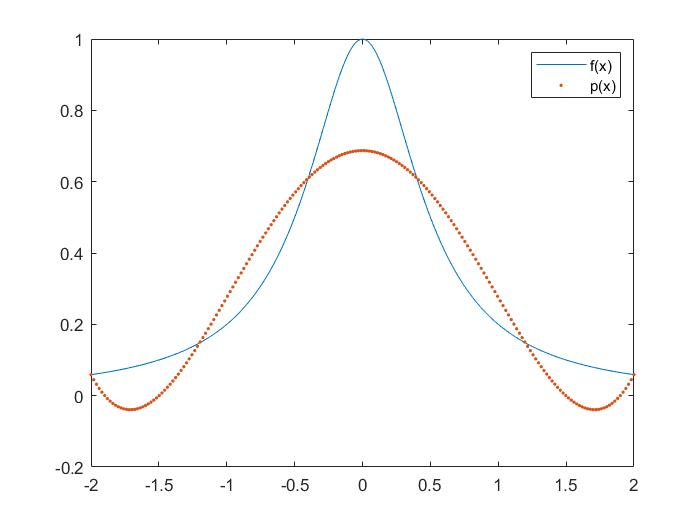
\includegraphics[width=8cm]{uniform6.jpg}
        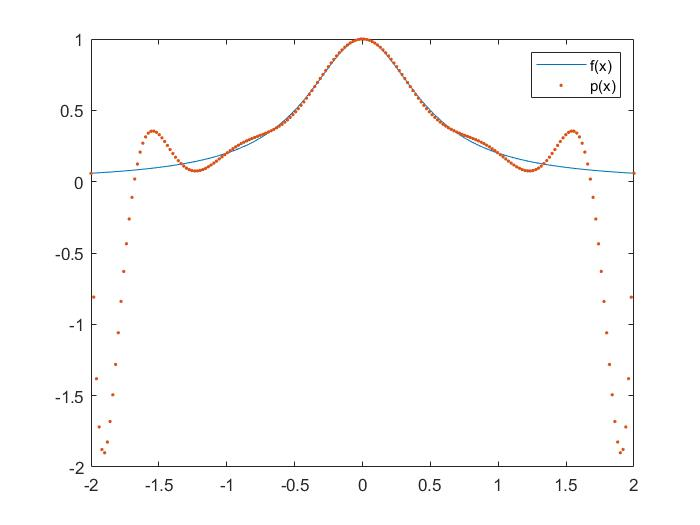
\includegraphics[width=8cm]{uniform13.jpg}  
  \end{figure}
  
  \item  
  Since the uniform distributed seems not good at some point, so we can use "Chebyshev nodes":
   \lstinputlisting[language=Matlab, numbers=left, stepnumber=1, firstline=1,caption={Chebyshev.m function},frame=single]{Chebyshev.m}
   And we can get the output
     \lstinputlisting[language=Matlab,caption={Output}]{Chebyshev.txt}
     
     And from the figure below, we can see that the polynomial meet much better to the original function than before, when we do it with uniform distributed nodes.
     
     \begin{figure}[ht]
        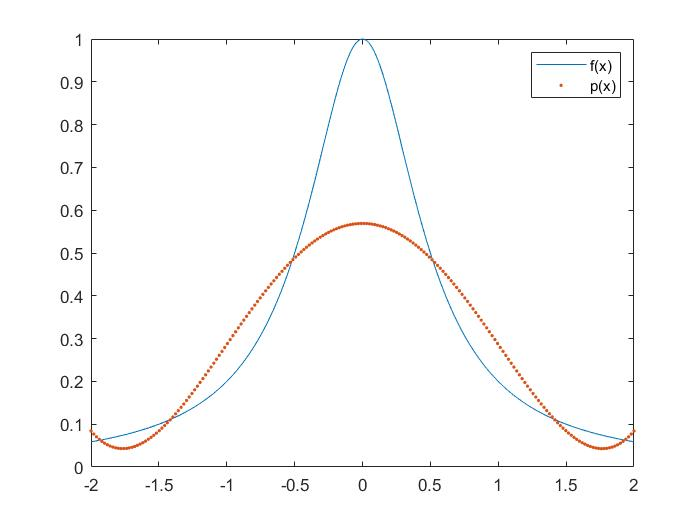
\includegraphics[width=8cm]{chebyshev6.jpg}
        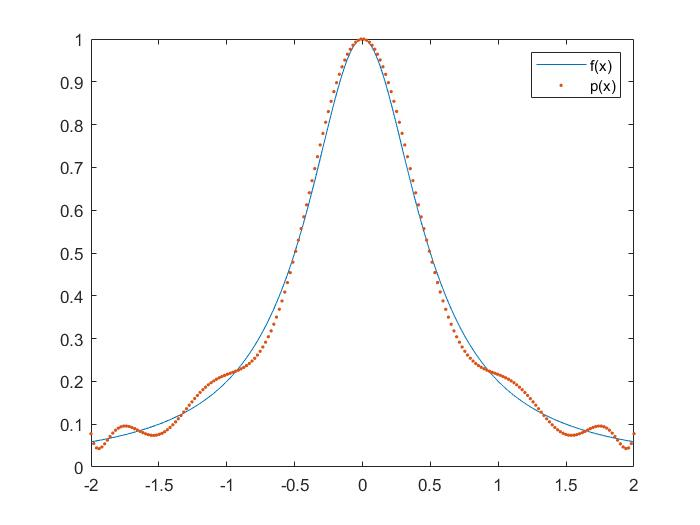
\includegraphics[width=8cm]{chebyshev13.jpg}
     \end{figure}
\end{enumerate}

\end{enumerate}
\end{document}